% \vspace{-1mm}
\section{Problem Statement}
%
% \begin{wrapfigure}{r}{0.4\textwidth} %this figure will be at the right
%     \vspace{-5mm}
%     \centering
%     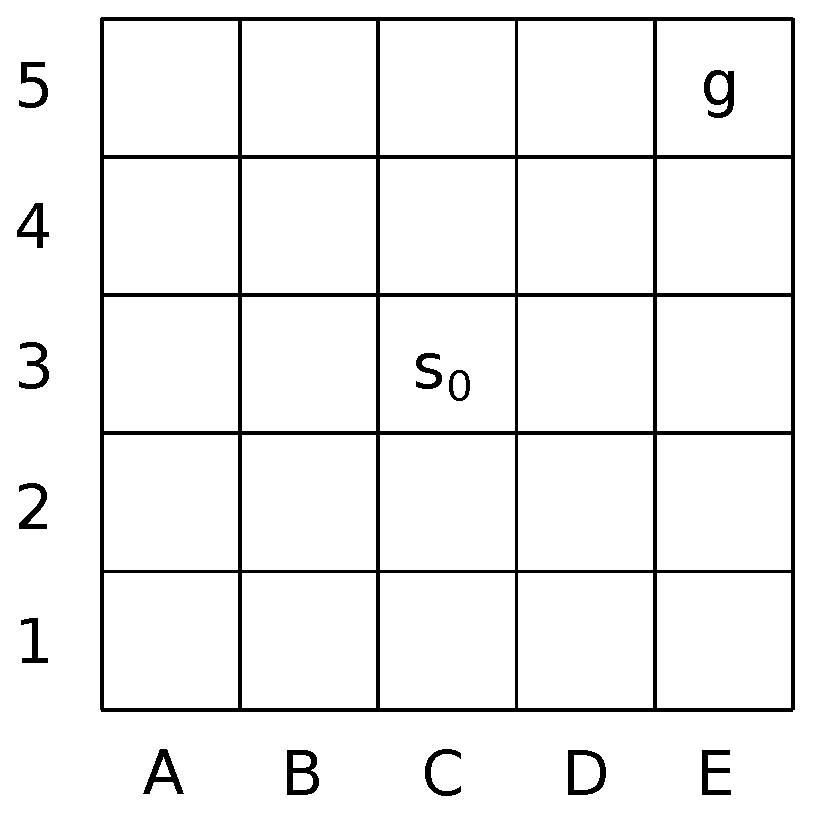
\includegraphics[width=0.25\textwidth]{./figures/drawing.eps}
%     \caption{Schematic of the problem}
%     \label{fig:schematic}
%     \vspace{-5mm}
% \end{wrapfigure}
%
I want to come up with a general procedure that solves the inverse kinematics
problem for redundant manipulators. Concretely, I will work with the planar
three-link articulated robot. I am only interested in the position of its
end-effector. Therefore, the forward kinematics map goes from the joint angles
$\theta = (\theta_1, \theta_2, \theta_3)$ to the end-effector position
$\mathrm{x} = (x,y)$. The problem is to find the inverse (one-to-many)
correspondence, i.e., the joint angles $\theta$ inducing a given end-effector
position $\mathrm{x}$.